\documentclass[aspectratio=169]{beamer}
\usetheme{metropolis}

\usepackage[utf8]{inputenc}
\usepackage{graphicx}
\usepackage{booktabs}
\usepackage{xcolor}
\usepackage{tikz}
\usepackage{amsmath}
\usepackage{amssymb}
\usepackage{tcolorbox}
\usepackage{array}
\usepackage{listings}
\usetikzlibrary{arrows.meta, positioning, calc, shapes.geometric}

%% ── COLOUR PALETTE ──────────────────────────────────────────
\definecolor{midnightblue}{RGB}{15, 28, 60}
\definecolor{techblue}{RGB}{32, 103, 178}
\definecolor{iceblue}{RGB}{180, 210, 245}
\definecolor{accentcyan}{RGB}{0, 188, 212}
\definecolor{accentgreen}{RGB}{76, 175, 80}
\definecolor{accentorange}{RGB}{255, 152, 0}
\definecolor{softgray}{RGB}{240, 242, 246}
\definecolor{darktext}{RGB}{20, 30, 55}

%% ── METROPOLIS COLOURS ──────────────────────────────────────
\setbeamercolor{normal text}    {fg=darktext, bg=white}
\setbeamercolor{frametitle}     {fg=white, bg=midnightblue}
\setbeamercolor{title separator}{fg=accentcyan}
\setbeamercolor{progress bar}   {fg=accentcyan, bg=iceblue}
\setbeamerfont{frametitle}      {size=\large, series=\bfseries}
\setbeamerfont{normal text}     {size=\small}

%% ── TCOLORBOX STYLES ────────────────────────────────────────
\tcbuselibrary{skins, breakable}
\tcbset{
  nbox/.style={
    colback=midnightblue!8, colframe=techblue,
    fonttitle=\bfseries\small, title=#1,
    left=4pt, right=4pt, top=3pt, bottom=3pt, boxrule=1.2pt, arc=3pt},
  rbox/.style={
    colback=accentgreen!10, colframe=accentgreen,
    fonttitle=\bfseries\small, title=#1,
    left=4pt, right=4pt, top=3pt, bottom=3pt, boxrule=1.2pt, arc=3pt},
  wbox/.style={
    colback=accentorange!10, colframe=accentorange,
    fonttitle=\bfseries\small, title=#1,
    left=4pt, right=4pt, top=3pt, bottom=3pt, boxrule=1pt, arc=3pt},
  gbox/.style={
    colback=softgray, colframe=darktext!30,
    fonttitle=\bfseries\small, title=#1,
    left=4pt, right=4pt, top=3pt, bottom=3pt, boxrule=0.8pt, arc=3pt}
}

%% ── CODE LISTINGS ───────────────────────────────────────────
\lstset{
  language=Python,
  basicstyle=\ttfamily\scriptsize,
  breaklines=true,
  frame=single,
  backgroundcolor=\color{softgray},
  keywordstyle=\color{techblue}\bfseries,
  commentstyle=\color{accentgreen!70!black}\itshape,
  stringstyle=\color{accentorange!80!black},
  numbers=none, tabsize=2,
  xleftmargin=3pt, xrightmargin=3pt
}

%% ── METADATA ────────────────────────────────────────────────
\title{Hindi Coreference Resolution\\for Low-Resource NLP}
\subtitle{Using Transformer-Based Hybrid Approaches\\[2pt]
          {\small B.Tech Final Year Project --- CIT Kokrajhar, May 2026}}
\author{Himraj Doley \quad Subham Saha \quad Mohd Zaid \quad Nipujyoti Rabha}
\institute{Dept.\ of Computer Science \& Engineering,
           Central Institute of Technology Kokrajhar\\
           \textit{Supervisor: Dr.\ Apurbalal Senapati (HOD, CSE)}}
\date{}

\setbeamertemplate{navigation symbols}{}

\begin{document}
\maketitle

% ════════════════════════════════════════════════════════
%  OUTLINE
% ════════════════════════════════════════════════════════
\begin{frame}{Presentation Outline}
  \begin{columns}[T]
    \column{0.48\textwidth}
      \begin{tcolorbox}[nbox={Sections 1 – 5}]
        \small
        \textbf{1.} Introduction\\[3pt]
        \textbf{2.} Motivation \& Objectives\\[3pt]
        \textbf{3.} Related Work\\[3pt]
        \textbf{4.} Methodology\\[3pt]
        \textbf{5.} Experimental Results
      \end{tcolorbox}
    \column{0.48\textwidth}
      \begin{tcolorbox}[nbox={Sections 6 – 9}]
        \small
        \textbf{6.} Contributions\\[3pt]
        \textbf{7.} Conclusion \& Limitations\\[3pt]
        \textbf{8.} Future Work\\[3pt]
        \textbf{9.} References
      \end{tcolorbox}
  \end{columns}
\end{frame}

% ════════════════════════════════════════════════════════
%  SECTION 1 — INTRODUCTION
% ════════════════════════════════════════════════════════
\section{Introduction}

\begin{frame}{What is Coreference Resolution?}
  \begin{tcolorbox}[nbox={Task Definition}]
    Identify \textbf{all referring expressions} in a text that point to the
    \textbf{same real-world entity} and group them into
    \textit{coreference chains} (entity clusters).
  \end{tcolorbox}

  \vspace{6pt}
  \begin{tcolorbox}[rbox={Hindi Example}]
    \centering\small
    \textit{``\textbf{Ram} school gaya.\ \textcolor{accentorange}{\textbf{Vah}} bahut khush tha.\
    \textcolor{accentorange}{\textbf{Usne}} doston se baat ki.''}\\[4pt]
    (Ram went to school.\ \textcolor{accentorange}{\textbf{He}} was happy.\
    \textcolor{accentorange}{\textbf{He}} talked to his friends.)\\[5pt]
    \textbf{Entity Cluster:} \{Ram,\ Vah,\ Usne\}
    $\longrightarrow$ all refer to the \emph{same person}
  \end{tcolorbox}

  \vspace{6pt}
  \begin{tcolorbox}[gbox={Why It Matters — Downstream Applications}]
    \centering\small
    Machine Translation $\;\cdot\;$ Question Answering $\;\cdot\;$ Summarisation\\[2pt]
    Dialogue Systems $\;\cdot\;$ Information Extraction $\;\cdot\;$ Knowledge Graphs
  \end{tcolorbox}
\end{frame}

\begin{frame}{Why Hindi? The Challenge}
  \begin{columns}[T]
    \column{0.52\textwidth}
      \begin{tcolorbox}[wbox={Hindi-Specific Challenges}]
        \small
        \begin{itemize}\setlength\itemsep{4pt}
          \item \textbf{Morphological richness:} Nouns, verbs, pronouns
                inflect for gender, number, case
          \item \textbf{Pro-drop behaviour:} Subject pronouns routinely omitted
          \item \textbf{Free word order:} SOV canonical, deviations common
          \item \textbf{Devanagari complexity:} Conjuncts, matras,
                zero-width joiners
          \item \textbf{Severe data scarcity:} No OntoNotes-scale resource
                for Hindi
        \end{itemize}
      \end{tcolorbox}

    \column{0.44\textwidth}
      \begin{tcolorbox}[rbox={The Scale of the Gap}]
        \small
        \renewcommand{\arraystretch}{1.35}
        \begin{tabular}{@{}ll@{}}
          \toprule
          \textbf{Language} & \textbf{Coref Data}\\
          \midrule
          English & ${\sim}10{,}000+$ docs\\
          Hindi   & ${\approx}0$ usable\\
          \bottomrule
        \end{tabular}\\[8pt]
        \textbf{Hindi speakers:}\\
        530M native $+$ 100M L2\\[5pt]
        \textcolor{red!70!black}{$\Rightarrow$ Critical NLP gap\\
        for 600M$+$ users}
      \end{tcolorbox}
  \end{columns}
\end{frame}

\begin{frame}{Our Two-Phase Research Journey}
  \begin{columns}[T]
    \column{0.48\textwidth}
      \begin{tcolorbox}[wbox={Phase 1 — Scratch BERT (Failed)}]
        \small
        \textbf{Approach:} Train BERT from scratch on 172K Hindi
        Wikipedia docs; cluster mentions by cosine similarity\\[6pt]
        \textbf{Result:} \textcolor{red!70!black}{\textbf{Systematic failure}}\\[3pt]
        Pronouns (\textit{vah, usne}) \emph{never} linked to
        correct antecedents at any threshold\\[6pt]
        \textbf{Root cause:} Coreference is \textbf{referential},
        not semantic — embedding similarity is structurally the
        wrong signal
      \end{tcolorbox}

    \column{0.48\textwidth}
      \begin{tcolorbox}[rbox={Phase 2 — Hybrid System (Succeeded)}]
        \small
        \textbf{Approach:} IndicBERTv2 contextual embeddings
        $+$ Hindi linguistic features
        $+$ Logistic Regression classifier
        $+$ Union-Find clustering\\[6pt]
        \textbf{Dataset:} 76 manually annotated Hindi documents
        (548 mention spans) — created from scratch\\[6pt]
        \textbf{Result:} ${\approx}$\textbf{82\%} pairwise accuracy\\
        \textcolor{accentgreen}{\textbf{$+$11 pp} from linguistic features}
      \end{tcolorbox}
  \end{columns}
  \vspace{6pt}
  \centering\small\textit{Phase 1 failure is documented as a principled
  negative result — itself a research contribution.}
\end{frame}


% ════════════════════════════════════════════════════════
%  SECTION 2 — MOTIVATION & OBJECTIVES
% ════════════════════════════════════════════════════════
\section{Motivation \& Objectives}

\begin{frame}{Motivation}
  \begin{columns}[T]
    \column{0.48\textwidth}
      \begin{tcolorbox}[nbox={The NLP Resource Gap}]
        \small
        \begin{itemize}\setlength\itemsep{4pt}
          \item Hindi = 3rd most-spoken language globally
          \item English coreference: OntoNotes 5.0 with
                \textit{thousands} of annotated docs
          \item Hindi coreference: effectively \textbf{zero}
                usable large-scale resources
          \item MT, QA, summarisation all hit a hard ceiling
                without coreference resolution
        \end{itemize}
      \end{tcolorbox}

      \vspace{6pt}
      \begin{tcolorbox}[wbox={Why Generic Models Fail}]
        \small
        mBERT / XLM-RoBERTa:\\[3pt]
        \textbullet\ Over-segment Devanagari text\\
        \textbullet\ Hindi signal diluted by 100$+$ languages\\
        \textbullet\ Never fine-tuned for Hindi coreference
      \end{tcolorbox}

    \column{0.48\textwidth}
      \begin{tcolorbox}[rbox={Three Research Questions}]
        \small
        \textbf{Q1.} Can embedding similarity alone resolve
        Hindi coreferences?\\
        \hfill\textcolor{red!70!black}{\textbf{No — and we explain why}}\\[6pt]
        \textbf{Q2.} Can a hybrid pipeline with IndicBERTv2
        work on just 76 docs?\\
        \hfill\textcolor{accentgreen}{\textbf{Yes}}\\[6pt]
        \textbf{Q3.} Do Hindi linguistic features add real value?\\
        \hfill\textcolor{accentgreen}{\textbf{$+$11 percentage points}}
      \end{tcolorbox}

      \vspace{6pt}
      \begin{tcolorbox}[nbox={Academic Value of Failure}]
        \small
        Documenting Phase 1 failure \textbf{saves future
        researchers} from repeating the same mistake
      \end{tcolorbox}
  \end{columns}
\end{frame}

\begin{frame}{Project Objectives}
  \begin{columns}[T]
    \column{0.48\textwidth}
      \begin{tcolorbox}[nbox={Primary Objectives}]
        \small
        \begin{enumerate}\setlength\itemsep{5pt}
          \item Evaluate limits of unsupervised
                embedding-based coreference
          \item Build a \textbf{functional end-to-end}
                Hindi coreference pipeline
          \item Create a \textbf{manually annotated}
                Hindi dataset (76 docs, 548 spans)
          \item Design a \textbf{hybrid architecture}
                combining IndicBERTv2 with
                hand-crafted Hindi features
        \end{enumerate}
      \end{tcolorbox}

    \column{0.48\textwidth}
      \begin{tcolorbox}[nbox={Technical Objectives}]
        \small
        \begin{itemize}\setlength\itemsep{4pt}
          \item Train SentencePiece BPE tokenizer
                (vocab = 32,000)
          \item Pretrain compact BERT-MLM on
                172K Hindi Wikipedia docs
          \item Extract IndicBERTv2 span embeddings
                (mean pooling)
          \item Engineer 11 Hindi-specific pairwise features
          \item Train Logistic Regression (5-fold CV,
                balanced weights)
          \item Union-Find cluster reconstruction
          \item Evaluate: Pairwise F1 $+$ MUC score
        \end{itemize}
      \end{tcolorbox}
  \end{columns}
\end{frame}


% ════════════════════════════════════════════════════════
%  SECTION 3 — RELATED WORK
% ════════════════════════════════════════════════════════
\section{Related Work}

\begin{frame}{Related Work — Language Models \& Indic NLP}
  \begin{columns}[T]
    \column{0.48\textwidth}
      \begin{tcolorbox}[nbox={Transformer Language Models}]
        \small
        \begin{itemize}\setlength\itemsep{5pt}
          \item \textbf{BERT} (Devlin et al., 2018)\\
                Bidirectional MLM; both directions matter for coref
          \item \textbf{RoBERTa} (Liu et al., 2019)\\
                More data $+$ no NSP $=$ better; explains why scratch model fails
          \item \textbf{Lauscher et al., 2020}\\
                Small pretrained models $\Rightarrow$ weaker representations; validates Phase 1 outcome
        \end{itemize}
      \end{tcolorbox}

    \column{0.48\textwidth}
      \begin{tcolorbox}[nbox={Indic Language Models}]
        \small
        \begin{itemize}\setlength\itemsep{5pt}
          \item \textbf{IndicBERT / IndicNLPSuite}
                (Kakwani et al., 2020)\\
                First systematic Indic NLP infrastructure
          \item \textbf{IndicBERTv2} (Doddapaneni et al., 2023)\\
                Larger IndicCorp v2; MLM-only; better Devanagari tokenisation\\
                \textcolor{accentgreen}{\textbf{$\rightarrow$ Our chosen backbone}}
          \item \textbf{MuRIL} (Khanuja et al., 2021)\\
                17 Indian languages; too large for our hardware
        \end{itemize}
      \end{tcolorbox}
  \end{columns}
\end{frame}

\begin{frame}{Related Work — Coreference Systems}
  \begin{columns}[T]
    \column{0.48\textwidth}
      \begin{tcolorbox}[nbox={Classical \& Statistical}]
        \small
        \begin{itemize}\setlength\itemsep{5pt}
          \item \textbf{Lappin \& Leass, 1994}\\
                Salience-based pronoun resolution;
                discourse proximity = key heuristic
          \item \textbf{Soon et al., 2001}\\
                Pairwise mention-pair model;
                \textit{conceptual basis for our classifier}
        \end{itemize}
      \end{tcolorbox}

      \vspace{6pt}
      \begin{tcolorbox}[nbox={Hindi-Specific}]
        \small
        \begin{itemize}\setlength\itemsep{4pt}
          \item \textbf{Mujadia et al., 2016}\\
                Guidelines $+$ small CoNLL Hindi dataset
          \item \textbf{Dakwale et al., 2013}\\
                Rule-based Hindi anaphora resolution
        \end{itemize}
      \end{tcolorbox}

    \column{0.48\textwidth}
      \begin{tcolorbox}[nbox={Neural Coreference}]
        \small
        \begin{itemize}\setlength\itemsep{5pt}
          \item \textbf{Lee et al., 2017}\\
                First end-to-end neural coref;
                joint mention $+$ antecedent scoring
          \item \textbf{Joshi et al., 2019 — SpanBERT}\\
                BERT spans for coref;
                80\%$+$ F1 on English OntoNotes
        \end{itemize}
      \end{tcolorbox}

      \vspace{6pt}
      \begin{tcolorbox}[wbox={The Resource Gap}]
        \small
        English (Lee/Joshi): \textbf{tens of thousands} of docs\\[3pt]
        Our Hindi system: \textbf{76 docs}\\[3pt]
        This gap \textbf{explains every design choice} we made
      \end{tcolorbox}
  \end{columns}
\end{frame}

\begin{frame}{Low-Resource NLP — Our Design Alignment}
  \vspace{2pt}
  \begin{tcolorbox}[nbox={Strategy $\longleftrightarrow$ Our Implementation}]
    \small
    \renewcommand{\arraystretch}{1.5}
    \begin{tabular}{p{3.5cm} p{3.8cm} p{4.0cm}}
      \toprule
      \textbf{Strategy} & \textbf{Literature} & \textbf{Our Implementation}\\
      \midrule
      Transfer learning & Hedderich et al., 2021 & IndicBERTv2 encoder backbone\\
      Feature engineering & Lappin \& Leass, 1994 & 11 Hindi pairwise features\\
      Simple classifiers & Hedderich et al., 2021 & Logistic Regression (not neural)\\
      Manual corpus creation & Hedderich et al., 2021 & 76 docs, 548 annotations\\
      \bottomrule
    \end{tabular}
  \end{tcolorbox}

  \vspace{8pt}
  \begin{tcolorbox}[rbox={Design Philosophy}]
    Every Phase 2 design decision is \textbf{grounded in the
    established low-resource NLP literature} — not an arbitrary choice.
  \end{tcolorbox}
\end{frame}


% ════════════════════════════════════════════════════════
%  SECTION 4 — METHODOLOGY
% ════════════════════════════════════════════════════════
\section{Methodology}

\begin{frame}{Phase 1 — Scratch BERT Setup}
  \begin{columns}[T]
    \column{0.48\textwidth}
      \begin{tcolorbox}[nbox={Corpus \& Tokenizer}]
        \small
        \textbf{Corpus:} 172,000 Hindi Wikipedia docs (Kaggle)\\[5pt]
        \textbf{Tokenizer:} SentencePiece BPE\\[4pt]
        \renewcommand{\arraystretch}{1.3}
        \begin{tabular}{@{}ll@{}}
          \toprule
          Algorithm    & BPE\\
          Vocab size   & 32,000\\
          Coverage     & 0.9995\\
          \bottomrule
        \end{tabular}\\[6pt]
        \textit{Why SentencePiece?} Operates on raw Unicode —
        no whitespace pre-tokenisation needed for Devanagari
      \end{tcolorbox}

    \column{0.48\textwidth}
      \begin{tcolorbox}[nbox={BERT Model Configuration}]
        \small
        Compact architecture (free-tier GPU):\\[4pt]
        \renewcommand{\arraystretch}{1.3}
        \begin{tabular}{@{}ll@{}}
          \toprule
          Hidden size    & 256\\
          Layers         & 4\\
          Attention heads& 4\\
          FFN size       & 512\\
          Max sequence   & 128 tokens\\
          Dropout        & 0.1\\
          \bottomrule
        \end{tabular}\\[6pt]
        \textbf{Objective:} MLM (15\% token masking), no NSP
      \end{tcolorbox}
  \end{columns}
\end{frame}

\begin{frame}{Phase 1 — Why It Failed}
  \begin{columns}[T]
    \column{0.50\textwidth}
      \begin{tcolorbox}[wbox={Failure Summary}]
        \small
        \renewcommand{\arraystretch}{1.35}
        \begin{tabular}{p{2.6cm} p{3.3cm}}
          \toprule
          \textbf{Failure} & \textbf{Observation}\\
          \midrule
          Pronoun linking & Not linked at \textit{any} threshold\\
          Threshold tuning & No good P-R trade-off\\
          Spurious clusters & Low threshold merges wrong spans\\
          Entity variation & Same entity unreliably merged\\
          Cross-sentence & No entity-tracking mechanism\\
          \bottomrule
        \end{tabular}
      \end{tcolorbox}

      \vspace{6pt}
      \begin{tcolorbox}[nbox={Key Metric}]
        \centering\small
        Precision on pronoun-antecedent pairs\\
        at cosine threshold 0.7:\\[4pt]
        \textcolor{red!70!black}{\Large\textbf{$< 30\%$}}\\[2pt]
        \small (barely above random chance)
      \end{tcolorbox}

    \column{0.46\textwidth}
      \begin{tcolorbox}[nbox={Root Cause Analysis}]
        \small
        \textbf{Ram} (proper noun) and \textbf{vah} (pronoun)
        have \textcolor{red!70!black}{\textbf{zero semantic similarity}}
        — yet are coreferent.\\[8pt]
        Coreference is \textbf{referential}, not semantic.\\[8pt]
        Embedding similarity detects semantic relatedness —
        which is \textbf{irrelevant} to referential identity.\\[8pt]
        This failure is \textit{systematic}: no amount of
        threshold tuning can fix it.
      \end{tcolorbox}

      \vspace{6pt}
      \begin{tcolorbox}[rbox={Outcome}]
        \small
        Phase 1 formally discontinued.\\
        Findings documented as a\\
        \textbf{principled negative result}.
      \end{tcolorbox}
  \end{columns}
\end{frame}


\begin{frame}{Phase 2 — Hybrid System Pipeline}
  \begin{columns}[T]
    \column{0.44\textwidth}
      \begin{tcolorbox}[nbox={4-Stage Pipeline}]
        \small
        \begin{enumerate}\setlength\itemsep{5pt}
          \item \textbf{Mention Representation}\\
                IndicBERTv2 mean-pooling over span tokens:
                $\mathbf{m}_{[i,j]}=\frac{1}{j{-}i{+}1}\sum_{k=i}^{j}\mathbf{h}_k$
          \item \textbf{Feature Construction}\\
                Embedding features $+$ 11 Hindi linguistic features
          \item \textbf{Pairwise Classification}\\
                Logistic Regression: coreferent vs.\ not
          \item \textbf{Cluster Reconstruction}\\
                Union-Find on predicted positive pairs
        \end{enumerate}
      \end{tcolorbox}

    \column{0.52\textwidth}
      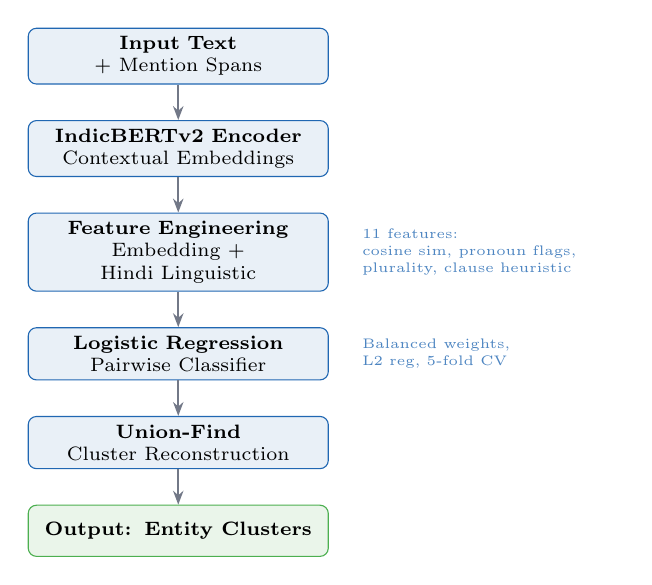
\begin{tikzpicture}[
        every node/.style={font=\scriptsize},
        node distance=0.45cm,
        box/.style={draw=techblue, fill=techblue!10, rounded corners=3pt,
                    minimum height=0.65cm, text width=3.6cm,
                    align=center, inner sep=3pt},
        outbox/.style={draw=accentgreen, fill=accentgreen!12, rounded corners=3pt,
                       minimum height=0.65cm, text width=3.6cm,
                       align=center, inner sep=3pt, font=\scriptsize\bfseries},
        arr/.style={-{Stealth[length=5pt]}, thick, darktext!60},
        ann/.style={font=\tiny, text=techblue!80, text width=3.2cm, align=left}
      ]
        \node[box]                 (A) {\textbf{Input Text}\\+ Mention Spans};
        \node[box, below=of A]     (B) {\textbf{IndicBERTv2 Encoder}\\Contextual Embeddings};
        \node[box, below=of B]     (C) {\textbf{Feature Engineering}\\Embedding + Hindi Linguistic};
        \node[box, below=of C]     (D) {\textbf{Logistic Regression}\\Pairwise Classifier};
        \node[box, below=of D]     (E) {\textbf{Union-Find}\\Cluster Reconstruction};
        \node[outbox, below=of E]  (F) {\textbf{Output: Entity Clusters}};

        \draw[arr] (A)--(B);
        \draw[arr] (B)--(C);
        \draw[arr] (C)--(D);
        \draw[arr] (D)--(E);
        \draw[arr] (E)--(F);

        \node[ann, right=0.3cm of C]
          {11 features:\\cosine sim, pronoun flags,\\plurality, clause heuristic};
        \node[ann, right=0.3cm of D]
          {Balanced weights,\\L2 reg, 5-fold CV};
      \end{tikzpicture}
  \end{columns}
\end{frame}

\begin{frame}{Dataset — Created Entirely From Scratch}
  \begin{columns}[T]
    \column{0.50\textwidth}
      \begin{tcolorbox}[wbox={No Public Hindi Coref Dataset Existed!}]
        \small
        The team annotated 76 documents manually over several weeks.
      \end{tcolorbox}

      \vspace{6pt}
      \small
      \renewcommand{\arraystretch}{1.4}
      \begin{tabular}{@{}ll@{}}
        \toprule
        \textbf{Property} & \textbf{Value}\\
        \midrule
        Total documents & 76\\
        Mention annotations & 548\\
        Avg.\ mentions / doc & 7.2\\
        Source domains & News, Wikipedia, Narratives\\
        Script & Devanagari (Hindi)\\
        Mention types & 4 categories\\
        \bottomrule
      \end{tabular}

      \vspace{6pt}
      \begin{tcolorbox}[nbox={Annotation Steps}]
        \small
        1.\ Read document fully\\
        2.\ Mark all coreferring NPs \& pronouns\\
        3.\ Assign shared cluster IDs\\
        4.\ Store as structured JSON
      \end{tcolorbox}

    \column{0.46\textwidth}
      \begin{tcolorbox}[nbox={Mention Type Taxonomy}]
        \small
        \renewcommand{\arraystretch}{1.35}
        \begin{tabular}{p{2.2cm} p{3.2cm}}
          \toprule
          \textbf{Type} & \textbf{Meaning}\\
          \midrule
          \texttt{proper\_noun}    & Named entity (person, org)\\
          \texttt{common\_noun}    & Definite/indefinite NP\\
          \texttt{pronoun}         & Personal/demonstrative\\
          \texttt{nominal\_phrase} & Descriptive NP by role\\
          \bottomrule
        \end{tabular}
      \end{tcolorbox}

      \vspace{6pt}
      \begin{tcolorbox}[wbox={Known Limitations}]
        \small
        $\bullet$\ Small size (76 documents)\\
        $\bullet$\ No formal inter-annotator agreement (Kappa)\\
        $\bullet$\ Skewed toward formal written Hindi\\[3pt]
        \textit{All honestly reported in the project report.}
      \end{tcolorbox}
  \end{columns}
\end{frame}


\begin{frame}{Hindi Linguistic Feature Engineering}
  \begin{columns}[T]
    \column{0.56\textwidth}
      \begin{tcolorbox}[nbox={Feature Vector for Mention Pair $(m_a,\,m_b)$}]
        \small
        \renewcommand{\arraystretch}{1.35}
        \begin{tabular}{p{3.0cm} p{4.0cm}}
          \toprule
          \textbf{Feature} & \textbf{Description}\\
          \midrule
          Cosine similarity & $\cos(\mathbf{m}_a,\mathbf{m}_b)$\\
          Embedding diff & $|\mathbf{m}_a - \mathbf{m}_b|$ (reduced)\\
          Pronoun flag ($m_a$) & 1 if \textit{vah, yah, main, hum, ve}\\
          Pronoun flag ($m_b$) & 1 if $m_b$ is a Hindi pronoun\\
          Object pronoun & 1 if \textit{use, inhe, unhe}\\
          Plural pronoun & 1 if \textit{ve, hum, ye}\\
          Sentence distance & Normalised mention gap\\
          Mention length ratio & $|m_a|\,/\,|m_b|$ (tokens)\\
          Clause heuristic & Same local subject clause?\\
          Head word match & Identical stem?\\
          Mention compatibility & Gender/number agreement\\
          \bottomrule
        \end{tabular}
      \end{tcolorbox}

    \column{0.40\textwidth}
      \begin{tcolorbox}[wbox={Why Not Embeddings Alone?}]
        \small
        \textit{Ram} (proper noun)\\
        $\leftrightarrow$ \textit{vah} (pronoun)\\[3pt]
        Share \textcolor{red!70!black}{\textbf{zero}} semantic overlap
        — yet clearly coreferent.\\[6pt]
        \textbf{Pronoun flag} signals:\\
        ``coreferent with proximate nominal''\\[4pt]
        \textbf{Plural flag} prevents:\\
        \textit{ve} (they) $\to$ singular antecedent
      \end{tcolorbox}

      \vspace{6pt}
      \begin{tcolorbox}[rbox={Ablation Preview}]
        \small
        Embedding only\hfill ${\approx}71\%$\\
        $+$ Linguistic features\hfill \textbf{${\approx}82\%$}\\[4pt]
        \centering
        \textcolor{accentgreen}{\large\textbf{$+11$ pp gain}}
      \end{tcolorbox}
  \end{columns}
\end{frame}

\begin{frame}[fragile]{Cluster Reconstruction — Union-Find}
  \begin{columns}[T]
    \column{0.52\textwidth}
      \begin{tcolorbox}[nbox={Python Implementation}]
\begin{lstlisting}
class UnionFind:
    def __init__(self, n):
        self.parent = list(range(n))

    def find(self, x):
        while self.parent[x] != x:
            self.parent[x] = \
              self.parent[self.parent[x]]
            x = self.parent[x]
        return x

    def union(self, x, y):
        px, py = self.find(x), self.find(y)
        if px != py:
            self.parent[px] = py

def build_clusters(mentions, pos_pairs):
    uf = UnionFind(len(mentions))
    for i, j in pos_pairs:
        uf.union(i, j)
    clusters = {}
    for idx in range(len(mentions)):
        clusters.setdefault(
          uf.find(idx),[]).append(mentions[idx])
    return list(clusters.values())
\end{lstlisting}
      \end{tcolorbox}

    \column{0.44\textwidth}
      \begin{tcolorbox}[rbox={How It Works}]
        \small
        \textbf{Step 1:} Each mention starts
        in its own singleton set\\[4pt]
        \textbf{Step 2:} For each predicted
        positive pair $(m_a,m_b)$: merge sets\\[4pt]
        \textbf{Step 3:} Connected components
        become entity clusters
      \end{tcolorbox}

      \vspace{6pt}
      \begin{tcolorbox}[wbox={Known Weakness}]
        \small
        \textbf{Transitive error propagation:}\\[3pt]
        If $m_a$--$m_b$ \emph{and} $m_b$--$m_c$ are
        both wrongly predicted coreferent,
        $m_a$ and $m_c$ get merged even though
        they should not.\\[3pt]
        One wrong prediction cascades through
        the cluster.
      \end{tcolorbox}

      \vspace{6pt}
      \begin{tcolorbox}[gbox={Compute Environment}]
        \small
        Platform: Google Colab / Kaggle\\
        GPU: T4 / P100 (free tier)\\
        Python 3.10; transformers, sklearn
      \end{tcolorbox}
  \end{columns}
\end{frame}


% ════════════════════════════════════════════════════════
%  SECTION 5 — EXPERIMENTAL RESULTS
% ════════════════════════════════════════════════════════
\section{Experimental Results}

\begin{frame}{Phase 1 Results — Embedding Experiments}
  \begin{columns}[T]
    \column{0.50\textwidth}
      \begin{tcolorbox}[nbox={Positive Observations}]
        \small
        Semantically coherent noun categories
        (body parts, country names, professions)
        showed \textbf{moderate spatial clustering}
        in embedding space.\\[5pt]
        Confirms MLM training captured
        some distributional structure.
      \end{tcolorbox}

      \vspace{6pt}
      \begin{tcolorbox}[wbox={Critical Failure — Pronouns}]
        \small
        Hindi pronouns (\textit{vah, yah, main, hum})
        formed a loose cluster, but:\\[4pt]
        $\bullet$\ No separation by number, case, or role\\
        $\bullet$\ No link to correct antecedents\\[6pt]
        \centering
        Precision on pronoun-antecedent pairs\\
        at threshold 0.7:\\[3pt]
        \textcolor{red!70!black}{\Large\textbf{$< 30\%$}}\\[2pt]
        \small Barely above random chance
      \end{tcolorbox}

    \column{0.46\textwidth}
      \begin{tcolorbox}[wbox={Failure Mode Summary}]
        \small
        \renewcommand{\arraystretch}{1.3}
        \begin{tabular}{p{2.5cm} p{3.0cm}}
          \toprule
          \textbf{Failure} & \textbf{Observation}\\
          \midrule
          Pronoun linking & Not linked at any threshold\\
          Threshold tuning & No good P-R balance\\
          Spurious clusters & Low threshold wrong merges\\
          Entity variation & Same entity not reliably merged\\
          Cross-sentence & No entity tracking\\
          \bottomrule
        \end{tabular}
      \end{tcolorbox}

      \vspace{6pt}
      \begin{tcolorbox}[rbox={Phase 1 Conclusion}]
        \small
        Failure is \textbf{systematic and fundamental}
        — not fixable by tuning.\\[3pt]
        Structural mismatch between task and method.\\[3pt]
        \textbf{Phase 1 formally discontinued.}
      \end{tcolorbox}
  \end{columns}
\end{frame}

\begin{frame}{Phase 2 Results — Classification Accuracy}
  \begin{columns}[T]
    \column{0.50\textwidth}
      \begin{tcolorbox}[nbox={Pairwise Classification (5-Fold CV)}]
        \small
        \renewcommand{\arraystretch}{1.4}
        \begin{tabular}{lccc}
          \toprule
          \textbf{Class} & \textbf{P} & \textbf{R} & \textbf{F1}\\
          \midrule
          Non-coref (0) & High & High & High\\
          \textcolor{accentorange}{\textbf{Coref (1)}} & Mod. & Mod. & Mod.\\
          \midrule
          \multicolumn{4}{c}{\textbf{Overall Accuracy:}
            \textcolor{accentorange}{\Large\textbf{${\approx}82\%$}}}\\
          \bottomrule
        \end{tabular}
      \end{tcolorbox}

      \vspace{6pt}
      \begin{tcolorbox}[nbox={Interpreting 82\%}]
        \small
        Non-coreferent pairs vastly outnumber
        coreferent pairs.\\[3pt]
        A ``predict-all-negative'' classifier
        would also score high.\\[3pt]
        Key: \textbf{genuine performance on the
        minority coreferent class} — achieved
        via balanced class weighting.
      \end{tcolorbox}

    \column{0.46\textwidth}
      \begin{tcolorbox}[rbox={Ablation Study}]
        \small\centering
        \renewcommand{\arraystretch}{1.4}
        \begin{tabular}{lc}
          \toprule
          \textbf{Feature Set} & \textbf{Acc.}\\
          \midrule
          Embedding only & ${\approx}71\%$\\
          \textbf{$+$ Linguistic features} & \textbf{${\approx}82\%$}\\
          \bottomrule
        \end{tabular}\\[6pt]
        \textcolor{accentgreen}{\Large\textbf{$+11$ pp}}\\[2pt]
        \small from pronoun flags, plurality\\
        and clause heuristics
      \end{tcolorbox}

      \vspace{6pt}
      \begin{tcolorbox}[nbox={MUC Coreference Evaluation}]
        \small
        \renewcommand{\arraystretch}{1.35}
        \begin{tabular}{lc}
          \toprule
          \textbf{System} & \textbf{MUC F1}\\
          \midrule
          Phase 1 (clustering) & Low\\
          \textbf{Phase 2 (ours)} & \textbf{Moderate}\\
          \bottomrule
        \end{tabular}\\[4pt]
        Clear cluster-level improvement
        over Phase 1 baseline.
      \end{tcolorbox}
  \end{columns}
\end{frame}

\begin{frame}{Qualitative Examples — Success \& Failure}
  \begin{tcolorbox}[rbox={Successful Resolution \checkmark}]
    \small
    \textbf{Input:}
    \textit{``Ram school gaya.\ Vah bahut khush tha.\ Usne apne doston se baat ki.''}\\
    \hspace{1.5em}(Ram went to school.\ He was very happy.\ He talked to his friends.)\\[4pt]
    \textbf{Gold:}\ \{Ram, Vah, Usne\}\quad
    \textbf{Predicted:}\ \{Ram, Vah, Usne\}\quad
    \textcolor{accentgreen}{\textbf{Correct}}\\[3pt]
    \textit{Why it worked:} Pronoun flags fired for \textit{Vah} and \textit{Usne};
    clause heuristic confirmed shared local subject with \textit{Ram}.
  \end{tcolorbox}

  \vspace{8pt}

  \begin{tcolorbox}[wbox={Failure Case $\boldsymbol{\times}$}]
    \small
    \textbf{Input:}
    \textit{``Seema aur Priya dono school gayi.\ Vah bahut thak gayi thi.''}\\
    \hspace{1.5em}(Seema and Priya both went to school.\ She was very tired.)\\[4pt]
    \textbf{Gold:}\ \{Seema aur Priya, Vah\}\ (collective)\ \quad
    \textbf{Predicted:}\ \{Seema, Vah\}\
    \textcolor{red!70!black}{\textbf{Incorrect}}\\[3pt]
    \textit{Why it failed:} Plurality check does not handle
    \textbf{conjoined noun phrases}; no collective antecedent tracking.
  \end{tcolorbox}
\end{frame}


% ════════════════════════════════════════════════════════
%  SECTION 6 — CONTRIBUTIONS
% ════════════════════════════════════════════════════════
\section{Contributions}

\begin{frame}{Key Contributions of This Project}
  \begin{columns}[T]
    \column{0.48\textwidth}
      \begin{tcolorbox}[rbox={Research Contributions}]
        \small
        \begin{enumerate}\setlength\itemsep{5pt}
          \item \textbf{Documented failure analysis}\\
                Explains \textit{why} embedding-based
                clustering fails for Hindi coref
          \item \textbf{Manually annotated dataset}\\
                76 docs, 548 spans, 4 types —
                created entirely from scratch
          \item \textbf{Working end-to-end pipeline}\\
                IndicBERTv2 $+$ Hindi features $+$
                LR $+$ Union-Find
        \end{enumerate}
      \end{tcolorbox}

    \column{0.48\textwidth}
      \begin{tcolorbox}[rbox={Empirical Contributions}]
        \small
        \begin{enumerate}\setlength\itemsep{5pt}
          \setcounter{enumi}{3}
          \item \textbf{Validated transfer learning}\\
                IndicBERTv2 outperforms scratch-trained
                model even at tiny fine-tuning scale
          \item \textbf{Feature importance evidence}\\
                Pronoun, plurality, clause features
                add \textcolor{red!70!black}{\textbf{$+$11 pp}}
                over embeddings alone
          \item \textbf{Honest evaluation}\\
                MUC $+$ pairwise F1 $+$ qualitative
                failure analysis reported transparently
        \end{enumerate}
      \end{tcolorbox}
  \end{columns}
\end{frame}

% ════════════════════════════════════════════════════════
%  SECTION 7 — CONCLUSION & LIMITATIONS
% ════════════════════════════════════════════════════════
\section{Conclusion \& Limitations}

\begin{frame}{Conclusion — What We Achieved}
  \begin{columns}[T]
    \column{0.50\textwidth}
      \begin{tcolorbox}[nbox={Results Summary}]
        \small
        \begin{itemize}\setlength\itemsep{4pt}
          \item \textbf{Phase 1} failed systematically;
                failure documented as a research finding
          \item \textbf{Phase 2} — functional Hindi
                coreference pipeline
          \item \textbf{${\approx}82\%$} overall pairwise accuracy
          \item \textbf{$+$11 pp} from Hindi linguistic features
          \item \textbf{MUC score} shows clear improvement
                over Phase 1 baseline
        \end{itemize}
      \end{tcolorbox}

      \vspace{6pt}
      \begin{tcolorbox}[rbox={Lessons Learned}]
        \small
        \textbf{L1:} Task formulation $>$ data volume\\[2pt]
        \textbf{L2:} Pretrained knowledge invaluable even at tiny scale\\[2pt]
        \textbf{L3:} Feature engineering still matters in transformer era\\[2pt]
        \textbf{L4:} Documenting failure = valid research\\[2pt]
        \textbf{L5:} Dataset creation = genuine contribution
      \end{tcolorbox}

    \column{0.46\textwidth}
      \begin{tcolorbox}[wbox={Limitations (Honestly Reported)}]
        \small
        \begin{enumerate}\setlength\itemsep{4pt}
          \item \textbf{Dataset size:} 76 docs is small;
                generalisation uncertain
          \item \textbf{No auto mention detection:}
                System needs pre-supplied spans
          \item \textbf{Classifier ceiling:}
                LR is linear; non-linear interactions missed
          \item \textbf{Union-Find transitivity:}
                One wrong pair cascades through cluster
          \item \textbf{Evaluation:} Only MUC $+$ pairwise;
                no B$^3$/CEAF; no CoNLL F1
          \item \textbf{No inter-annotator agreement}
                (Kappa not measured)
        \end{enumerate}
      \end{tcolorbox}
  \end{columns}
\end{frame}

% ════════════════════════════════════════════════════════
%  SECTION 8 — FUTURE WORK
% ════════════════════════════════════════════════════════
\section{Future Work}

\begin{frame}{Future Work — Prioritised Roadmap}
  \begin{columns}[T]
    \column{0.48\textwidth}
      \begin{tcolorbox}[nbox={High Priority}]
        \small
        \begin{enumerate}\setlength\itemsep{5pt}
          \item \textbf{Automatic Mention Detection}\\
                Fine-tune IndicBERTv2 as BIO labeller\\
                $\Rightarrow$ True end-to-end pipeline
          \item \textbf{Neural Pairwise Scorer}\\
                Replace LR with FFN or fine-tuned IndicBERTv2\\
                $\Rightarrow$ Break the linear ceiling
          \item \textbf{Dataset Expansion}\\
                76 $\to$ 300–500 docs; Cohen's Kappa ${\geq}0.7$;\\
                diversify domains; publish open-source
        \end{enumerate}
      \end{tcolorbox}

    \column{0.48\textwidth}
      \begin{tcolorbox}[nbox={Medium \& Long-Term}]
        \small
        \begin{enumerate}\setlength\itemsep{5pt}
          \setcounter{enumi}{3}
          \item \textbf{Full CoNLL Evaluation}\\
                B$^3$ $+$ CEAF via \texttt{coval}\\
                $\Rightarrow$ Cross-system comparison
          \item \textbf{Morphological Analyser}\\
                Explicit gender/number labels\\
                $\Rightarrow$ Fix plurality failures
          \item \textbf{SpanBERT-style Architecture}\\
                (Lee et al.\ $+$ IndicBERTv2 backbone)
          \item \textbf{Cross-lingual Transfer}\\
                Zero-shot from English OntoNotes
          \item \textbf{Downstream Integration}\\
                Hindi QA, summarisation, KG construction
        \end{enumerate}
      \end{tcolorbox}
  \end{columns}
\end{frame}

% ════════════════════════════════════════════════════════
%  SECTION 9 — REFERENCES
% ════════════════════════════════════════════════════════
\section{References}

\begin{frame}{References}
  \begin{columns}[T]
    \column{0.50\textwidth}
      \begin{tcolorbox}[gbox={Language Models \& Tools}]
        \scriptsize
        $[1]$ Devlin et al.\ (2018). BERT. \textit{arXiv:1810.04805}\\
        $[2]$ Liu et al.\ (2019). RoBERTa. \textit{arXiv:1907.11692}\\
        $[3]$ Lauscher et al.\ (2020). Zero-to-hero. \textit{EMNLP}\\
        $[4]$ Wolf et al.\ (2020). HuggingFace. \textit{EMNLP Demo}
      \end{tcolorbox}

      \vspace{5pt}
      \begin{tcolorbox}[gbox={Indic Language Models}]
        \scriptsize
        $[5]$ Kakwani et al.\ (2020). IndicNLPSuite. \textit{EMNLP}\\
        $[6]$ Doddapaneni et al.\ (2023). IndicBERTv2. \textit{arXiv}\\
        $[7]$ Khanuja et al.\ (2021). MuRIL. \textit{arXiv}
      \end{tcolorbox}

      \vspace{5pt}
      \begin{tcolorbox}[gbox={Hindi NLP}]
        \scriptsize
        $[8]$ Mujadia et al.\ (2016). Hindi coref. \textit{COLING}\\
        $[9]$ Dakwale et al.\ (2013). Hindi anaphora. \textit{IJCNLP}
      \end{tcolorbox}

    \column{0.46\textwidth}
      \begin{tcolorbox}[gbox={Coreference Systems}]
        \scriptsize
        $[10]$ Lappin \& Leass (1994). \textit{Comp.\ Ling.}\\
        $[11]$ Soon et al.\ (2001). ML coref. \textit{CL 27(4)}\\
        $[12]$ Lee et al.\ (2017). E2E coref. \textit{EMNLP}\\
        $[13]$ Joshi et al.\ (2019). SpanBERT. \textit{TACL 8}\\
        $[14]$ Vilain et al.\ (1995). MUC scoring. \textit{MUC-6}\\
        $[15]$ Moosavi \& Strube (2016). Metrics. \textit{ACL}
      \end{tcolorbox}

      \vspace{5pt}
      \begin{tcolorbox}[gbox={Low-Resource NLP}]
        \scriptsize
        $[16]$ Hedderich et al.\ (2021). Survey. \textit{NAACL}
      \end{tcolorbox}
  \end{columns}
\end{frame}

% ════════════════════════════════════════════════════════
%  THANK YOU
% ════════════════════════════════════════════════════════
\begin{frame}
  \vspace{0.4cm}
  \begin{center}
    {\Huge\bfseries\color{midnightblue} Thank You}\\[0.6cm]
    {\large\color{darktext!70} Questions \& Discussion}
  \end{center}

  \vspace{0.5cm}
  \begin{columns}[c]
    \column{0.52\textwidth}
      \begin{tcolorbox}[nbox={Project Summary}]
        \small
        \textbf{Task:} Hindi Coreference Resolution\\[3pt]
        \textbf{System:} IndicBERTv2 $+$ Hindi Features
        $+$ LR $+$ Union-Find\\[3pt]
        \textbf{Dataset:} 76 docs, 548 spans (from scratch)\\[3pt]
        \textbf{Result:} ${\approx}82\%$ pairwise accuracy\\[3pt]
        \textbf{Key finding:} Linguistic features $+$11 pp
        over embeddings alone
      \end{tcolorbox}

    \column{0.44\textwidth}
      \begin{tcolorbox}[rbox={Team}]
        \small
        Himraj Doley \hfill 202202023131\\
        Subham Saha \hfill 202202021067\\
        Mohd Zaid \hfill 202202023127\\
        Nipujyoti Rabha \hfill 202202021053\\[5pt]
        \textit{Supervisor:}\\
        Dr.\ Apurbalal Senapati (HOD, CSE)\\[3pt]
        CIT Kokrajhar — May 2026
      \end{tcolorbox}
  \end{columns}
\end{frame}

\end{document}
